\documentclass[UTF8]{article}
\usepackage{geometry}                % See geometry.pdf to learn the layout options. There are lots.
\geometry{a4paper}                   % ... or a4paper or a5paper or ... 

%\geometry{landscape}                % Activate for for rotated page geometry
\usepackage{graphicx}
\usepackage{hyperref}
\usepackage{amssymb}
\usepackage{epstopdf}
\usepackage{algorithm}
\usepackage[noend]{algpseudocode}
\usepackage{enumitem}
\usepackage[acronym]{glossaries}
\usepackage[hang,footnotesize,bf]{caption}
\DeclareGraphicsRule{.tif}{png}{.png}{`convert #1 `dirname #1`/`basename #1 .tif`.png}


% Copied from Stack Exchange for ToDo items
% -----------------------------------------------------------
\usepackage{xargs} 
\usepackage[pdftex,dvipsnames]{xcolor}  % Coloured text etc.
% 
\usepackage[colorinlistoftodos,prependcaption,textsize=tiny]{todonotes}
\newcommandx{\unsure}[2][1=]{\todo[linecolor=red,backgroundcolor=red!25,bordercolor=red,#1]{#2}}
\newcommandx{\change}[2][1=]{\todo[linecolor=blue,backgroundcolor=blue!25,bordercolor=blue,#1]{#2}}
\newcommandx{\info}[2][1=]{\todo[linecolor=OliveGreen,backgroundcolor=OliveGreen!25,bordercolor=OliveGreen,#1]{#2}}
\newcommandx{\improvement}[2][1=]{\todo[linecolor=Plum,backgroundcolor=Plum!25,bordercolor=Plum,#1]{#2}}
\newcommandx{\thiswillnotshow}[2][1=]{\todo[disable,#1]{#2}}


\title{Validator Economics: Variable min validator deposit size\\
\vspace{4pt}
\large EF Academic Grant ID: FY23-1030\\
\vspace{16pt}
DATA SOURCES \& GATHERING}
\vspace{16pt}
\author{Sandra Johnson\\
ConsenSys Software R\&D}
\date{\today}                                           % Activate to display a given date or no date

\begin{document}
\maketitle


% Acronym definitions
\newacronym{apr}{APR}{annual percentage rate}
\newacronym{ef}{EF}{Ethereum Foundation}
\newacronym{mev}{MEV}{maximal extractable value}
\newacronym{rig}{RIG}{Rigorous Incentives Group}
\newacronym{ssf}{SSF}{single slot finality}

% ------------------------------------------------------------------------------
\section{Overview}
% ------------------------------------------------------------------------------
This document is joint work with Kerrie Mengersen and Patrick O'Callaghan, and details available information, data sources, and proposed visualisations that will provide relevant data insights to gain a deeper understanding of current validator economics and any intuitions or assumptions used in formulating proposed solutions to capping the number of validators. 

The information gathering is targeted towards the proposal being evaluated, viz. a variable minimum validator balance, which is one of the proposals that Vitalik articulated in his blog post regarding \gls{ssf} 

As the project progresses and additional data requirements are identified, this document will be updated accordingly.

Many people have generously contributed time and data, and made helpful suggestions, which has been incredibly helpful in compiling the resources listed in this document. They include, but are not limited to Barnabé Monnot and the \gls{rig} team, Justin Drake, Alexander Tesfamichael, Ben Edgington, Paul Harris and Josh Fernandez.



\section{Data}
% ==================
\label{sec:data}

% ------------------------------
\subsection{Data Sources}
% ------------------------------
\label{sec:sources}
\begin{itemize}
	\item \textbf{Diversity - client, staking pools}
	\begin{itemize}
		\item \textit{\href{https://clientdiversity.org/}{Diversify Now}} dashboard by \textit{\href{https://etheralpha.org/}{Ether alpha}} displays the current client distribution in the Consensus and Execution layers.
		\item \textit{\href{https://migalabs.es/beaconnodes}{Beacon Chain Network Public Dashboard}} by \textit{\href{https://migalabs.es/}{Miga Labs}} has several visualisations: 
		\begin{itemize}
		\item Client diversity,  
		\item Client diversity evolution (Beacon chain client distribution over time)
		\item Active nodes
		\item Graphical distribution (Beacon chain node distribution)
		\item RTT distribution
	\end{itemize}
However, it is important to note that it is challenging to measure peer types in the network, and therefore the figures are at best approximations made based on the information at hand. 
	\end{itemize}
        \item \textbf{Ether Supply}
        \begin{itemize}
		\item \textit{\href{https://ultrasound.money/}{Ultra sound money}} visualises various aspects of Ether supply since the Merge, gas, supply projections, the burn, total value secured - TVS and monetary premium. \\
Ultrasound supplied two datasets - the first had total supply at a more accurate and finer grained level, but shorter time period and the second dataset had data points roughly every 1,000 epochs covering from soon after Beacon chain genesis. The latter dataset is from Glassnode and would not be as accurate as the initial data provided by Alex Tesfamichael from Ultrasound.
		\item \textit{\href{https://etherscan.io/chart/ethersupplygrowth}{Etherscan}} is a good source of historic data for the growth in Ether supply since 2015.
	\end{itemize}
	\item \textbf{Multiple data sources}
	\begin{itemize}
		\item \textit{\href{https://mevboost.pics/data.html}{Mevboost.pics - Open Data}} will eventually provide links to download several datasets: 
			\begin{itemize}
			\item \textit{eth\_data} - Slots since Merge with additional MEV-Boost and validator info such as: date, slot, block number, relay, builder pubkey, proposer pubkey, mevboost value, builder, validator \textit{(Available now)}
			\item \textit{pubkey\_mapping} - Validator public keys mapped to known entities such as Lido, Kraken ect. \textit{(Not available)}
			\item \textit{tc\_txs} - Tornado Cash related transactions \textit{(Not available)}
			\item \textit{staking\_txs} - Deposit transactions to the ETH2 Deposit contract \textit{(Not available)}
			\item \textit{relays\_over\_time} - Number of successfully relayed blocks per day \textit{(Not available)}
			\item \textit{builders\_over\_time} - Number of successfully built blocks per day \textit{(Not available)}
		\end{itemize}
	\end{itemize}
\end{itemize}

% ---------------------------------------------------------------
\subsection{Key data points}
% --------------------------------------------------------------
\begin{itemize}
\item The beacon chain \textbf{deposit contract address} is: 0x00000000219ab540356cBB839Cbe05303d7705Fa 
\item The beacon chain \textbf{genesis block number} is 11182202
\end{itemize}

% ---------------------------------------------------------------
\subsection{Existing visualisations}
% --------------------------------------------------------------
\subsubsection*{Client diversity}
% --------------------------------------
\begin{figure}[htbp]
\begin{center}
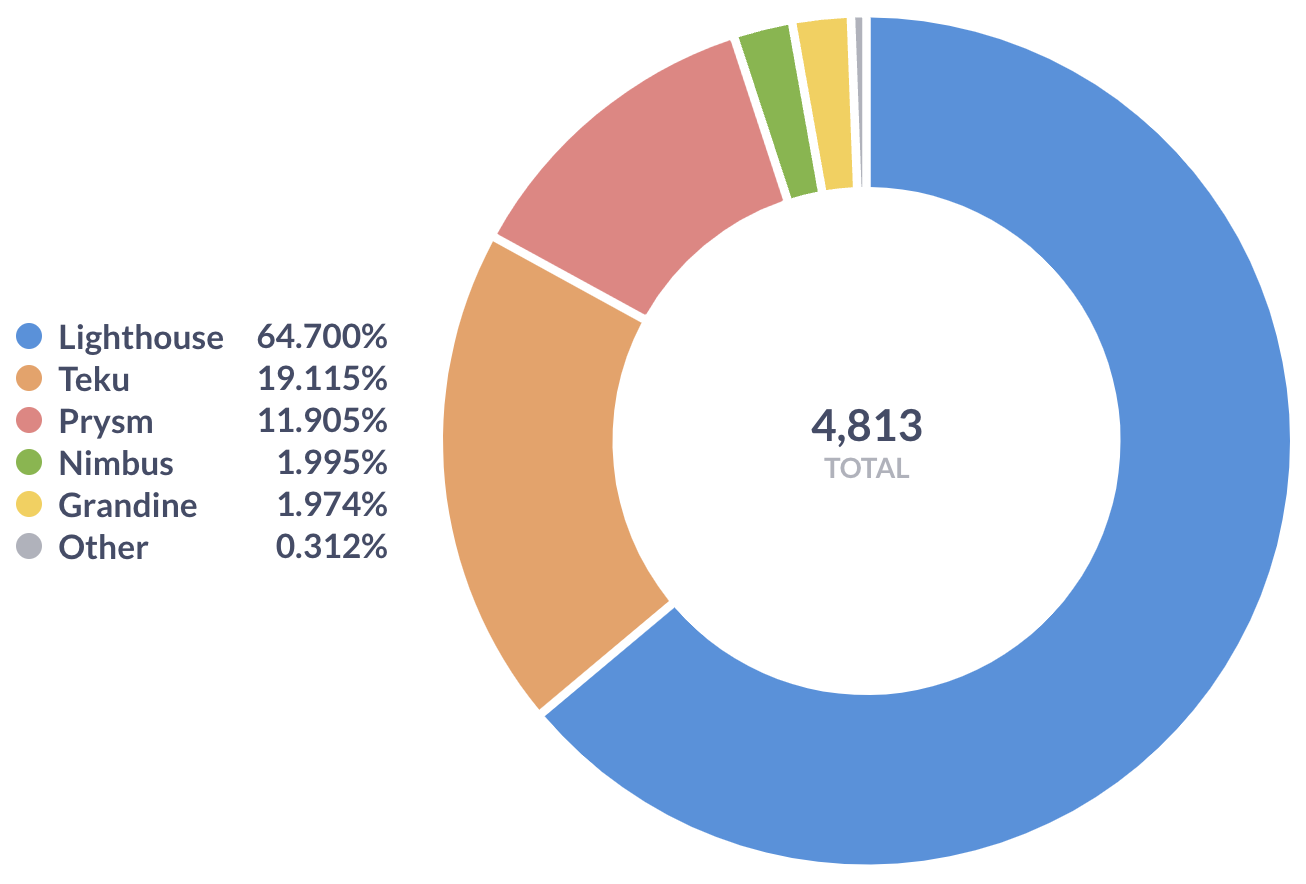
\includegraphics[width=0.4\linewidth]{images/clientdiversity}
\caption{Consensus layer client diversity by Migalabs (29 March 2023)}
\label{fig:migalabs}
\end{center}
\end{figure}

 \begin{figure}[htbp]
\begin{center}
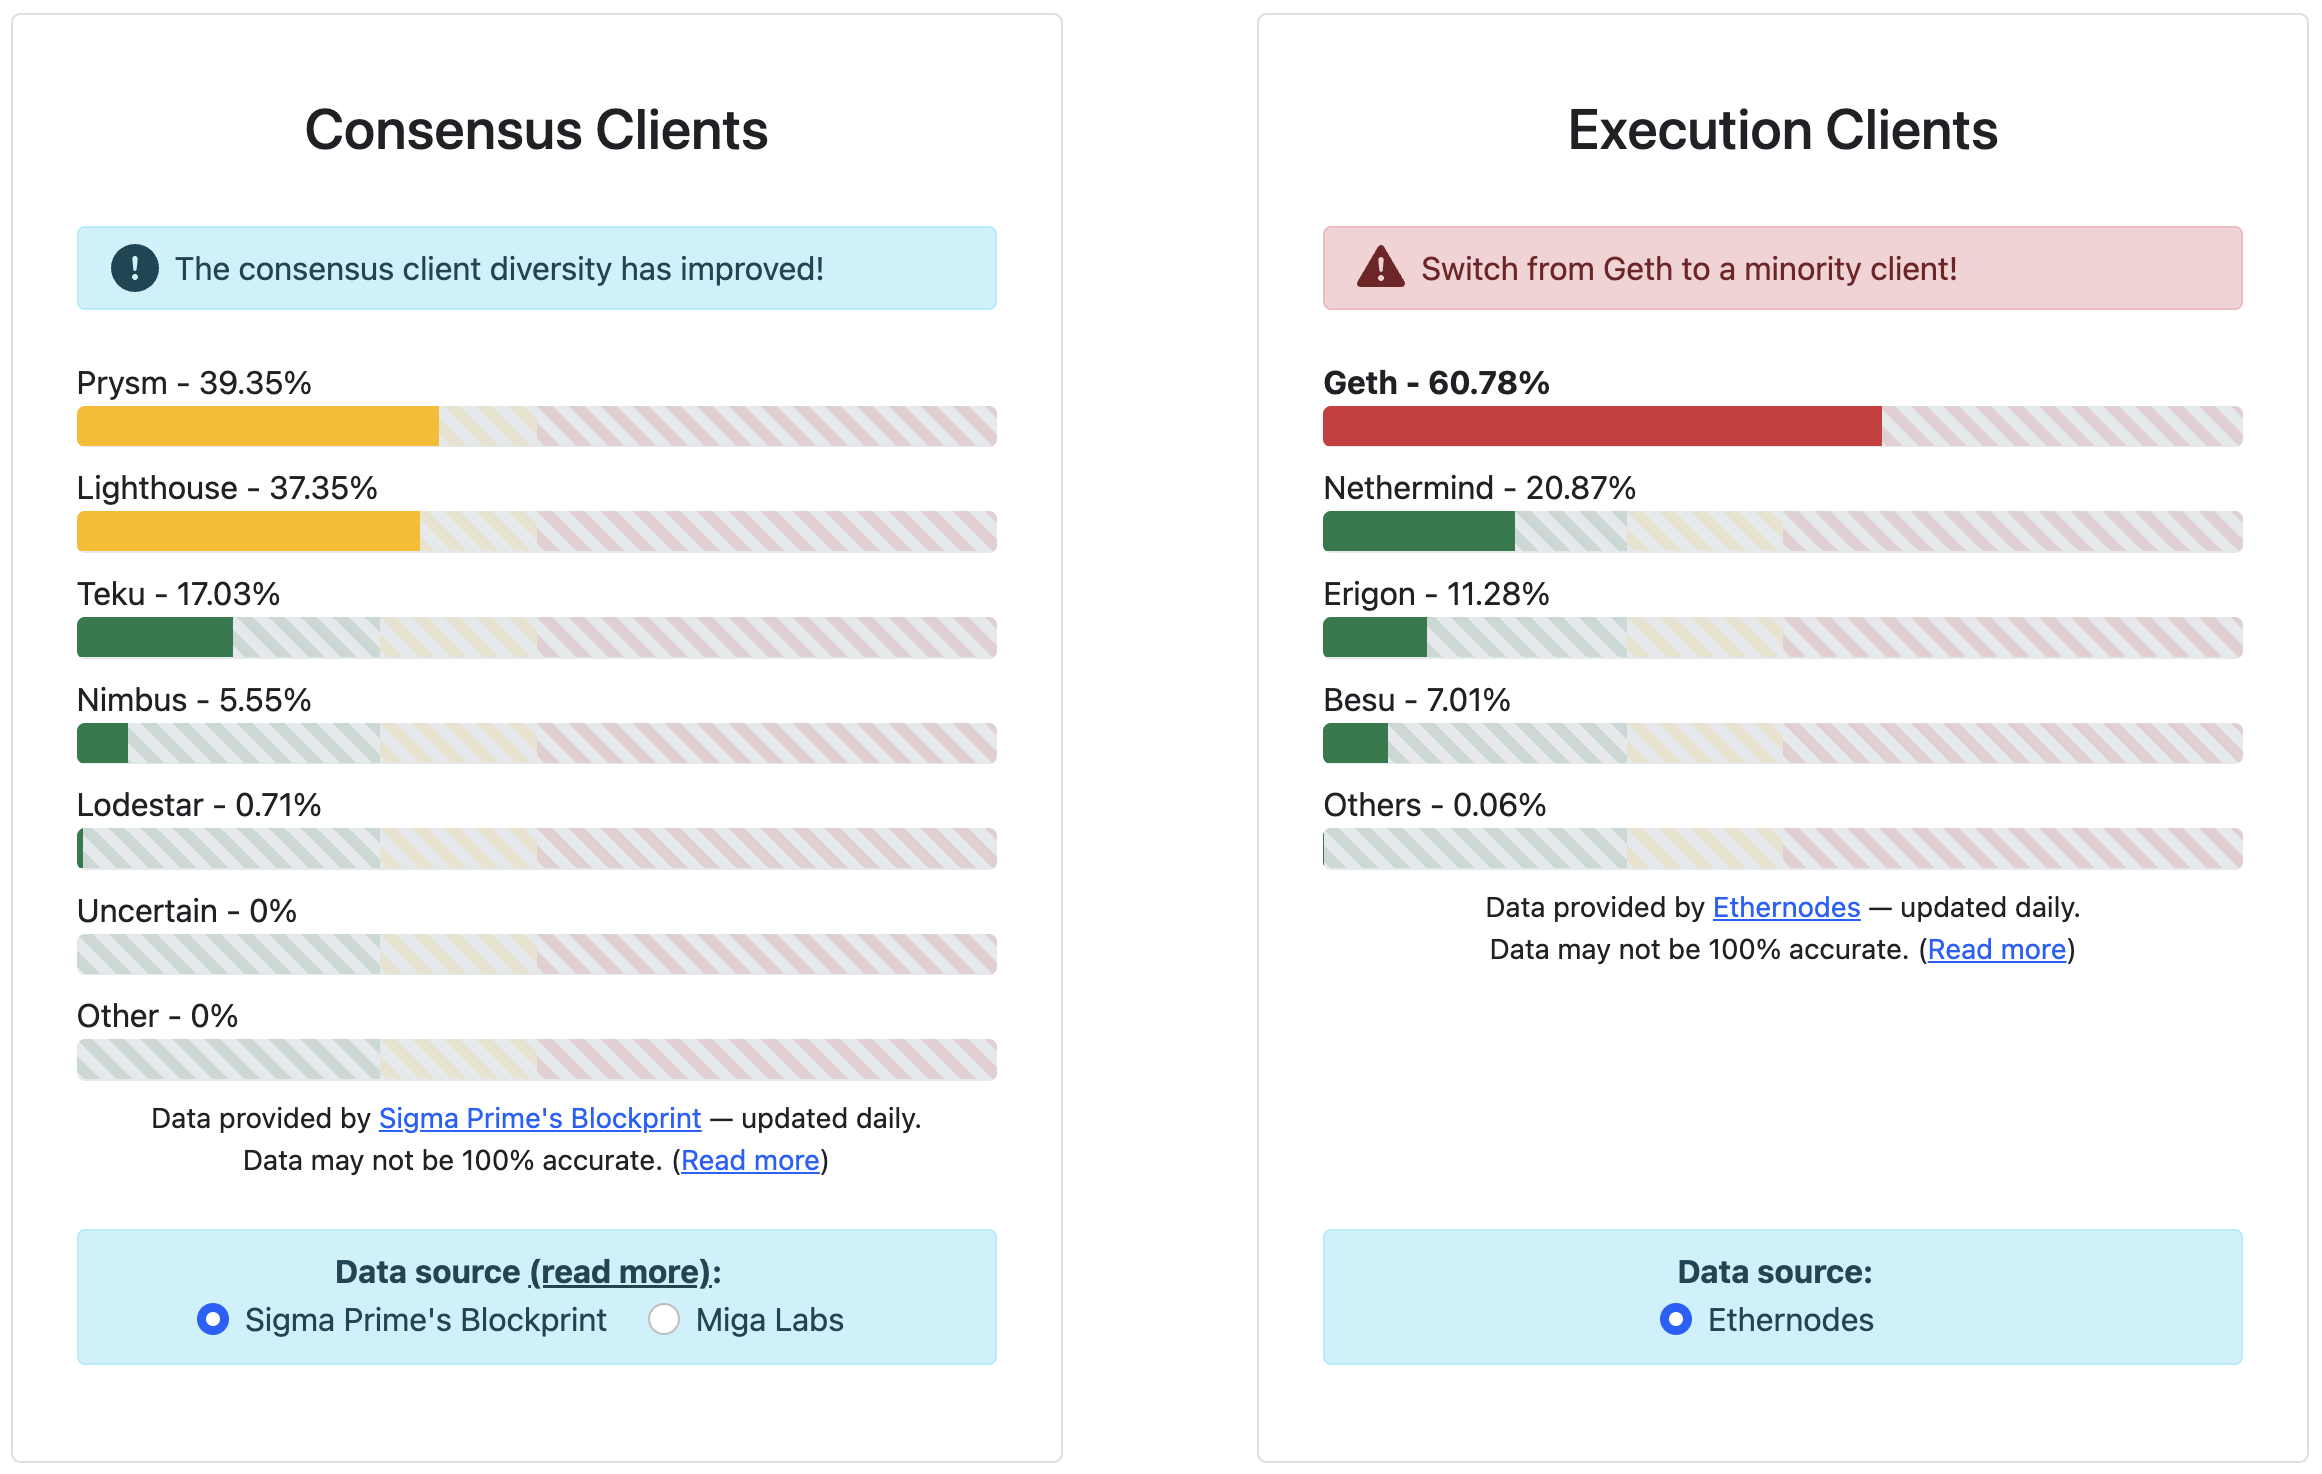
\includegraphics[width=0.9\linewidth]{images/clientdiversitysigma}
\caption{Consensus layer client diversity by Ether Alpha using a Sigma data source(29 March 2023)}
\label{fig:sigmaprime}
\end{center}
\end{figure}
\end{document}


